% -*-latex-*-
%\documentclass[pdftex,handout]{beamer}
\documentclass[pdftex,12pt]{beamer}
\usepackage{etex}

\let\latexput\put
\usepackage{pictex}
\let\pictexput\put
\let\put\latexput

\usepackage{color}
%\usepackage{pst-plot,color,pstricks}
%\setlength{\topmargin}{-1.7in}
\setbeamertemplate{footline}[frame number]
\begin{document}

\title{Neutral Evolution at Two Loci}
\author{Alan R. Rogers}
\date{\today}
\frame{\titlepage}

\begin{frame}
\frametitle{Linkage disquilibrium (LD)}
\begin{columns}
\column{0.35\textwidth}
\centering
\begin{tabular}{ccc}
       & \multicolumn{2}{c}{Locus}\\
Gamete &  1 & 2\\ \hline
 1&A&B\\
 2&A&B\\
 3&A&B\\
 4&A&B\\
 5&A&B\\
 6&A&b\\
 7&a&B\\
 8&a&B\\
 9&a&b\\
10&a&b\\
\end{tabular}
\column{0.65\textwidth}
\pause
{\centering
\begin{tabular}{c|cc|c}
 \multicolumn{1}{c}{} & A & \multicolumn{1}{c}{a}\\
\cline{2-3}
B & 5 & 2 & 7\\
b & 1 & 2 & 3\\
\cline{2-3}
\multicolumn{1}{c}{}
  & 6 & \multicolumn{1}{c}{4} & 10
\end{tabular}\\}
\pause
\begin{itemize}
\item $B$ is more common among $A$-gametes than $a$-gametes.
\pause
\item $A$ is more common among $B$-gametes than $b$-gametes.
\pause
\item This is LD.
\end{itemize}
\end{columns}
\end{frame}

\begin{frame}
Linkage disequilibrium (LD) is one of those unfortunate terms that
does not reveal its meaning. As every instructor of population
genetics knows, the term is a barrier not an aid to
understanding\ldots Detecting LD does not ensure either linkage or a
lack of equilibrium.\\ \mbox{}\hfill\small(Montgomery Slatkin, 2008)
\end{frame}

\begin{frame}
\frametitle{Linkage equilibrium (LE)}
\begin{columns}
\column{0.35\textwidth}
\centering
\begin{tabular}{ccc}
       & \multicolumn{2}{c}{Locus}\\
Gamete &  1 & 2\\ \hline
 1&A&B\\
 2&A&B\\
 3&A&B\\
 4&A&B\\
 5&A&b\\
 6&A&b\\
 7&a&B\\
 8&a&B\\
 9&a&b\\
\end{tabular}
\column{0.65\textwidth}
{\centering
\begin{tabular}{c|cc|c}
 \multicolumn{1}{c}{} & A & \multicolumn{1}{c}{a}\\
\cline{2-3}
B & 4 & 2 & 6\\
b & 2 & 1 & 3\\
\cline{2-3}
\multicolumn{1}{c}{}
  & 6 & \multicolumn{1}{c}{3} & 9
\end{tabular}\\}
\pause
\begin{itemize}
\item $B$ is equally common among $A$-gametes and $a$-gametes.
\pause
\item $A$ is equally common among $B$-gametes and $b$-gametes.
\pause
\item This is LE.
\end{itemize}
\end{columns}
\end{frame}

\begin{frame}
\frametitle{Linkage Equilibrium $\Longleftrightarrow$ shaded fractions equal}
\centering
\begin{columns}
\column{0.7\textwidth}
\let\put\pictexput
\mbox{\beginpicture
\setcoordinatesystem units <2cm,2cm>
\setplotarea x from 0 to 3.8, y from 0.0 to 2.4
\put {\makebox(0,0)[c]{\large $A$-gametes}} at 1 2.2
\put {\large $b$} at 1 1.5
\put {\large $B$} at 1 0.5
\circulararc 360 degrees from 2.000000 1.000000 center at 1.000000 1.000000
\plot 1.000000 1.000000 0.292893 0.292893 /
\plot 1.000000 1.000000 1.707107 0.292893 /
\setshadesymbol <z,z,z,z> ({.})
\setshadegrid span <3.5pt> point at 1.000000 1.000000
\vshade
0.292893 0.292893 0.292893
0.500000 0.133975 0.500000
0.741181 0.034074 0.741181
1.000000 0.000000 1.000000
1.258819 0.034074 0.741181
1.500000 0.133975 0.500000
1.707107 0.292893 0.292893
/
\put {\makebox(0,0)[c]{\large $a$-gametes}} at 3 2
\put {\large $b$} at 3 1.4
\put {\large $B$} at 3 0.6
\circulararc 360 degrees from 3.800000 1.000000 center at 3.000000 1.000000
\plot 3.000000 1.000000 2.434315 0.434315 /
\plot 3.000000 1.000000 3.565685 0.434315 /
\setshadesymbol <z,z,z,z> ({\large .})
\setshadegrid span <3.5pt> point at 3.000000 1.000000
\vshade
2.434315 0.434315 0.434315
2.600000 0.307180 0.600000
2.792945 0.227259 0.792945
3.000000 0.200000 1.000000
3.207055 0.227259 0.792945
3.400000 0.307180 0.600000
3.565685 0.434315 0.434315
/
\endpicture}
\let\put\latexput

\column{0.35\textwidth}\raggedright
LE: Knowledge about one locus tells nothing about other.

\bigskip

Here, $b$ is equally common among $a$-gametes and $A$-gametes.

\bigskip

(Also, $a$ is equally common among $b$-gametes and $B$-gametes.)
\end{columns}
\end{frame}

\begin{frame}
\frametitle{LD $\Longleftrightarrow$ shaded fractions unequal}
\centering
\begin{columns}
\column{0.7\textwidth}
\let\put\pictexput
\mbox{\beginpicture
\setcoordinatesystem units <2cm,2cm>
\setplotarea x from 0 to 3.8, y from 0.0 to 2.4
\put {\makebox(0,0)[c]{\large $A$-gametes}} at 1 2.2
\put {\large $B$} at 1 1.5
\put {\large $b$} at 1 0.5
\put {\makebox(0,0)[c]{\large $a$-gametes}} at 3 2
\put {\large $B$} at 3 1.4
\put {\large $b$} at 3 0.6
\circulararc 360 degrees from 2.000000 1.000000 center at 1.000000 1.000000
\plot 1.000000 1.000000 0.292893 0.292893 /
\plot 1.000000 1.000000 1.707107 0.292893 /
\setshadesymbol <z,z,z,z> ({.})
\setshadegrid span <3.5pt> point at 1.000000 1.000000
\vshade
0.292893 0.292893 0.292893
0.500000 0.133975 0.500000
0.741181 0.034074 0.741181
1.000000 0.000000 1.000000
1.258819 0.034074 0.741181
1.500000 0.133975 0.500000
1.707107 0.292893 0.292893
/
\circulararc 360 degrees from 3.800000 1.000000 center at 3.000000 1.000000
\plot 3.000000 1.000000 2.600000 0.307180 /
\plot 3.000000 1.000000 3.400000 0.307180 /
\setshadesymbol <z,z,z,z> ({.})
\setshadegrid span <3.5pt> point at 3.000000 1.000000
\vshade
2.600000 0.307180 0.307180
2.726384 0.248246 0.526083
2.861081 0.212154 0.759386
3.000000 0.200000 1.000000
3.138919 0.212154 0.759386
3.273616 0.248246 0.526083
3.400000 0.307180 0.307180
/
\endpicture}
\let\put\latexput

\column{0.35\textwidth}\raggedright
LD: Knowledge about one locus helps predict the other.

\bigskip

Here, $b$ is more common among $A$-gametes than among $a$-gametes.

\bigskip

(Also, $a$ is more common among $B$-gametes than among $b$-gametes.)
\end{columns}
\end{frame}

\begin{frame}
\frametitle{People sometimes confuse LD with epistasis}
\centering
\begin{tabular}{lp{0.6\textwidth}}
Epistasis & In a comparison of diploid genotypes, the \emph{phenotypic
  effect} of one locus depends on another locus.\\
Linkage disequilibrium & In a comparison of haploid chromosomes, the
\emph{allele frequency} at one locus depends on another locus.\\
\end{tabular}\\
\end{frame}

\begin{frame}
\frametitle{You can see LD in sequence data}
\begin{columns}
\column{0.6\textwidth}
 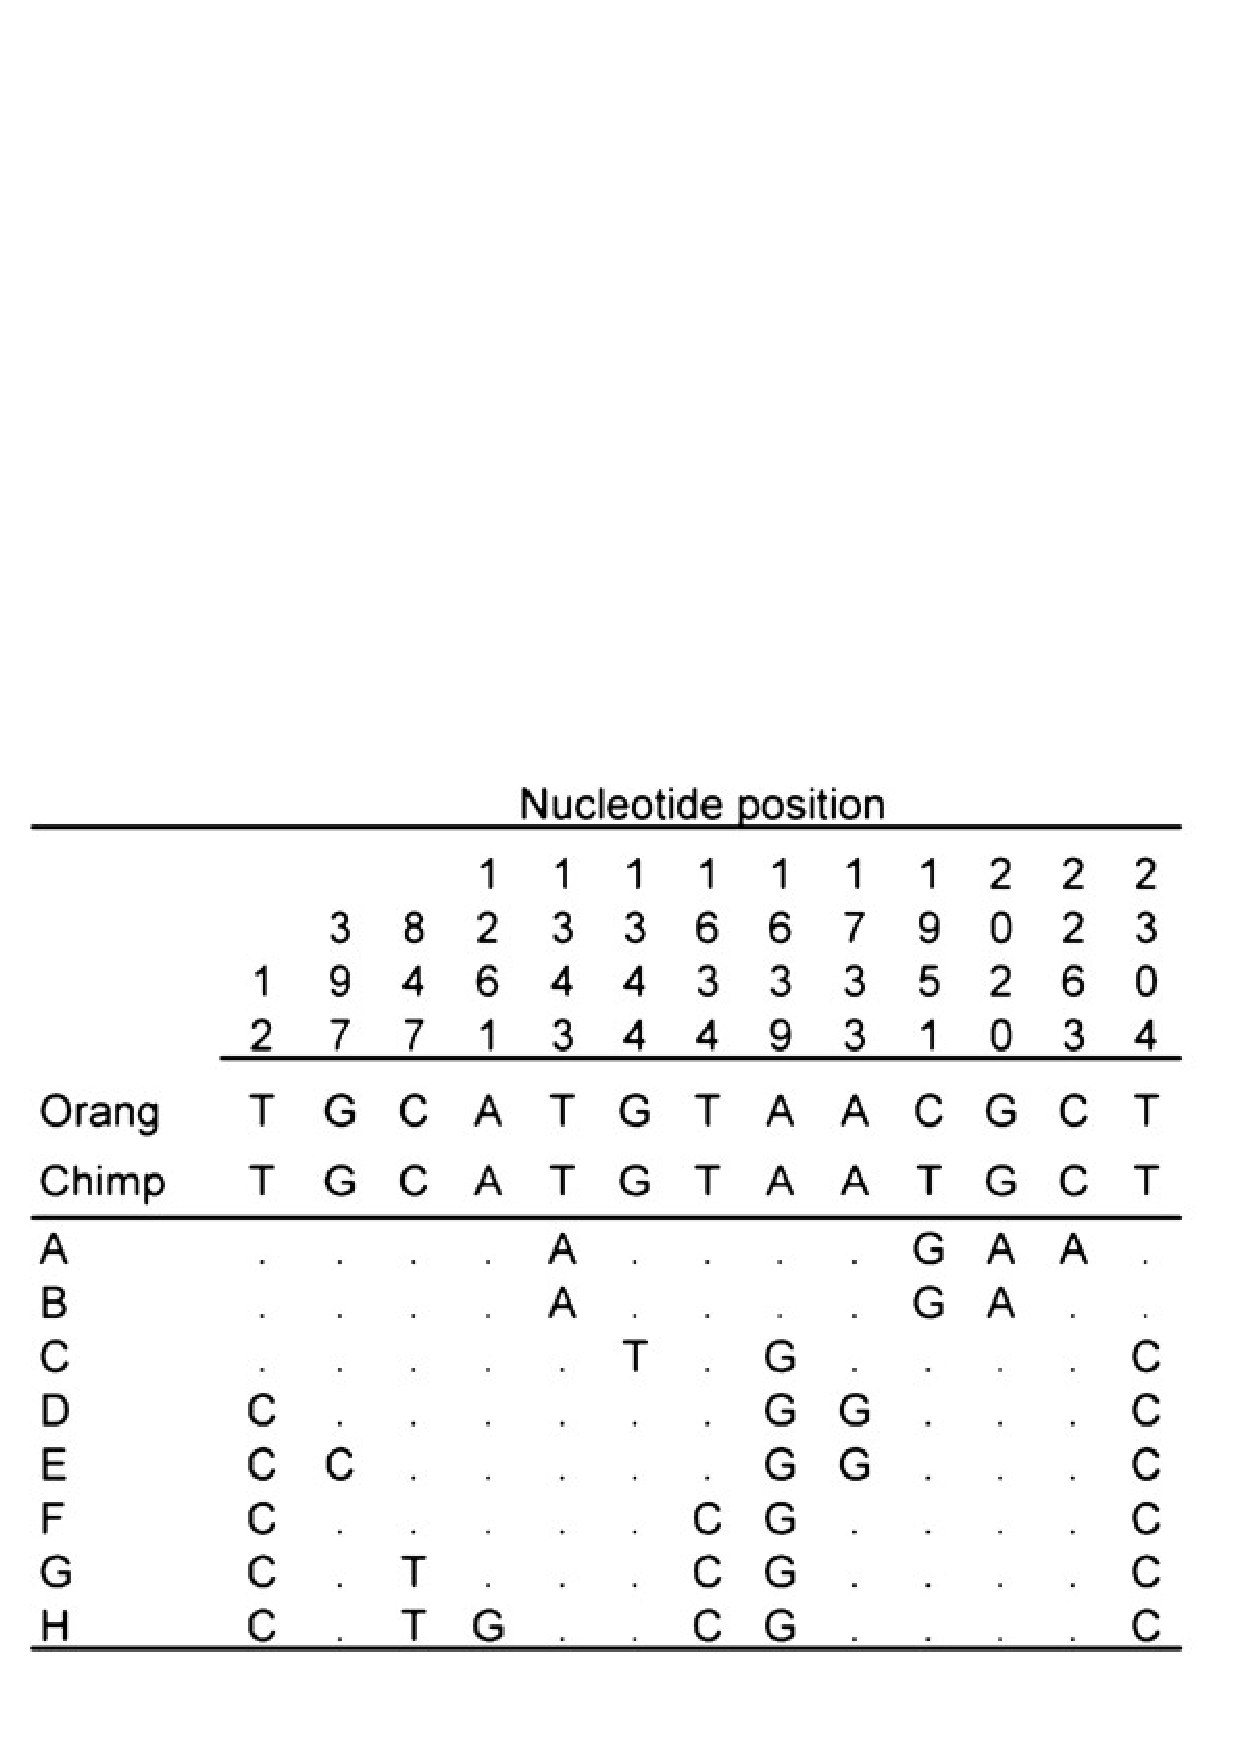
\includegraphics[width=\textwidth]{rrm2p4seq.png}\\
\textsc{\footnotesize (Garrigan et al 2004)}
\column{0.4\textwidth}\raggedright
\begin{itemize}
\item Dots: identical to chimp sequence.
\item Sites not independent.
\item A at site 1343 predicts G at 1951
\item This is linkage disequilibrium (LD).
\end{itemize}
\end{columns}
\end{frame}

\begin{frame}
\begin{columns}
\column{0.6\textwidth}
 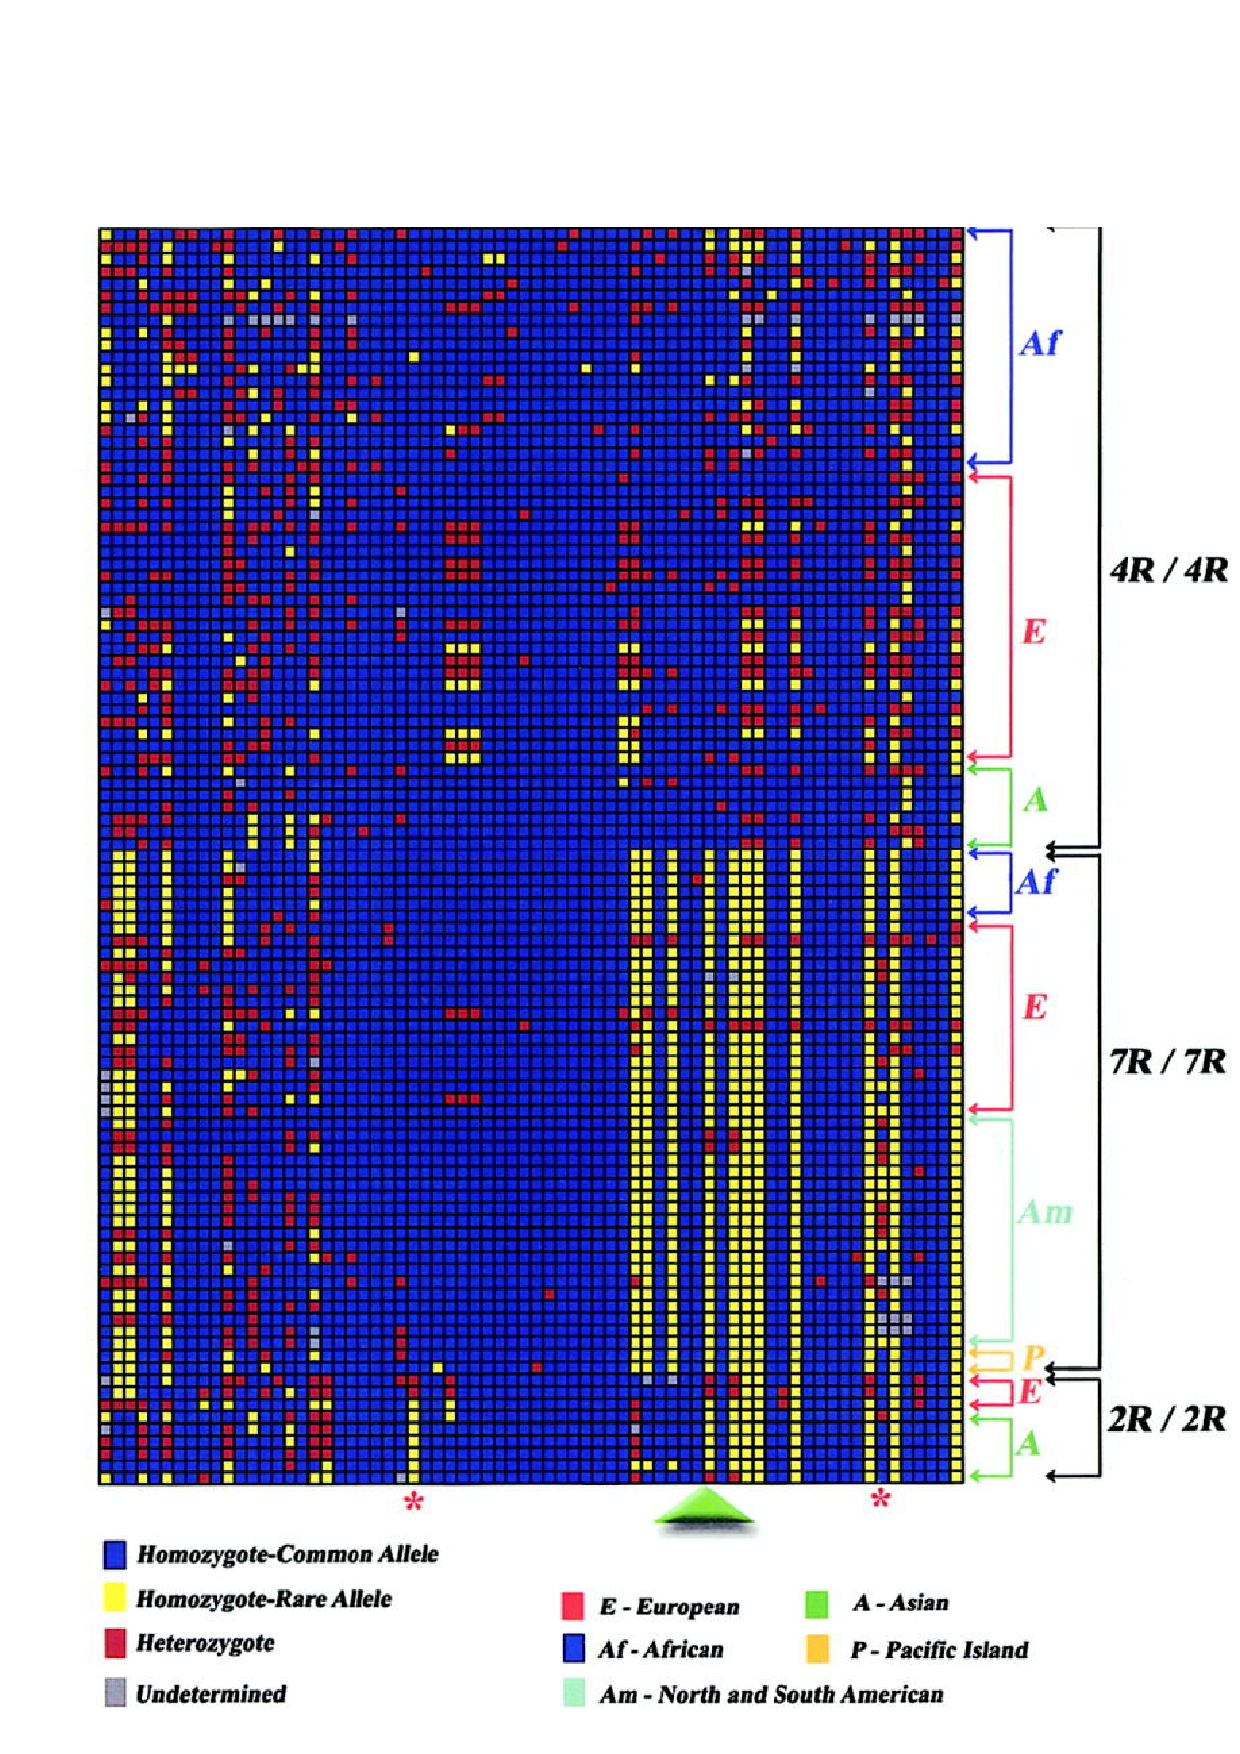
\includegraphics[height=0.9\textheight]{drd4-polymorph.pdf}
\column{0.4\textwidth}\raggedright
\begin{itemize}
\item Columns are SNPs
\item Rows are diploid genotypes
\item Blue: common homozygote
\item Yellow: rare homozygote
\item Red: heterozygote
\item Note LD w/i 7R genotypes
\end{itemize}
\end{columns}
\end{frame}

\begin{frame}
\frametitle{LD at the NF1 locus (Schmegner et al 2005)}
\includegraphics[width=\textwidth]{NF1.png}
\end{frame}

\begin{frame}
\frametitle{DNA sequences from region of human lactase gene}
%DNA sequences near human lactase gene, typed in a
%European sample.  Columns are
%nucleotide sites.  Top row (the
%reference sequence) shows common state at each site. Capital
%\texttt{A} is lactase persistance
%allele\cite{Bersaglieri:AJH-74-1111}.  Numbered rows represent
%individual chromosomes. Dots indicate identity with top row.  60
%chromosomes identical to reference sequence were omitted to save
%space. From HapMap release r23.}\label{tab.lctseq}
%
\tiny
\centering
\ttfamily
\begin{tabular}{cc}
  &cgcttcaggcattcctatctaaacagaccaacgtaAgggtacaatgcctaacccagacgtttcaactct\\
20&.....................................................................\\
21&.....................................................................\\
22&.....................................................................\\
23&.....................................................................\\
24&.....................................................................\\
25&.....................................................................\\
26&.....................................................................\\
27&..................t..................................................\\
28&..................t..................................................\\
29&..................................................c..................\\
37&...................................G..a.gt.....t.........gac.c.tgtct.\\
38&...ccgga....gat..at..gg..c.....tc.gGaaa.g..ccttt...tg......c...t.t...\\
39&...ccgga....gat..at..gg..c.....tc.gGaaa.g..ccttt...tg......c...t.t...\\
40&..tcc...agtag.t.cat..g.....t..ttccgG..a.gt.....t.........gac.c.tgtct.\\
41&..tcc...agtag.t.cat..g.....t.gttccgG..a.gt.....t.........gac.c.tgtct.\\
42&..tcc...agtag.t.cat..g.....t.gttccgG..a.gt.....t.........gac.c.tgtct.\\
43&..tcc...agtag.t.cat..g.....t.g.tc.gG..a.gt.....t.........gac.c.tgtct.\\
44&..tcc...agtag.t.cat..g.....t..ttc.gG..acgt.....t.........gac.c.tgtct.\\
45&..tcc...agtag.t.cat..g.....t.gttc.gG..a.gt.....t.........gac.c.tgtct.\\
46&...ccgga....gat..at..gg..c.....tc.gGaaa.g..ccttt...tg......cg.gt.t..c\\
47&..tcc...agtag.t.cat..g.....t.gttccgG..a.gt.....t.........gac.c.tgtct.\\
48&..tcc...agtag.t.cat..g.....t.gttccgG..a.gt.....t.........gac.c.tgtct.\\
49&..tcc...agtag.t.cat..g.....t.gttccgG..a.gt.....t.........gac.c.tgtct.\\
50&tatccgga....g.tc.atcgg.tc.g.tg.tc.gG..a.g.g....tg....ggt...cg.gt.t..c\\
51&ta.ccgga....g.t..atcgg.tc.g.tg.tc.gG..a.g.g....tg....ggt...cg.gt.t..c\\
52&ta.ccgga....g.t..atc.g.tc.g.tg.tc.gG..a.g.g....tg....ggt...cg.gt.t..c\\
53&ta.ccgga....g.t..atcgg.tc.g.tg.tc.gG..a.g.g....tg....ggt...cg.gt.t..c\\
\end{tabular}
\end{frame}

\begin{frame}
\frametitle{More LD in Europe than Africa}
\begin{columns}
\column{0.6\textwidth}
 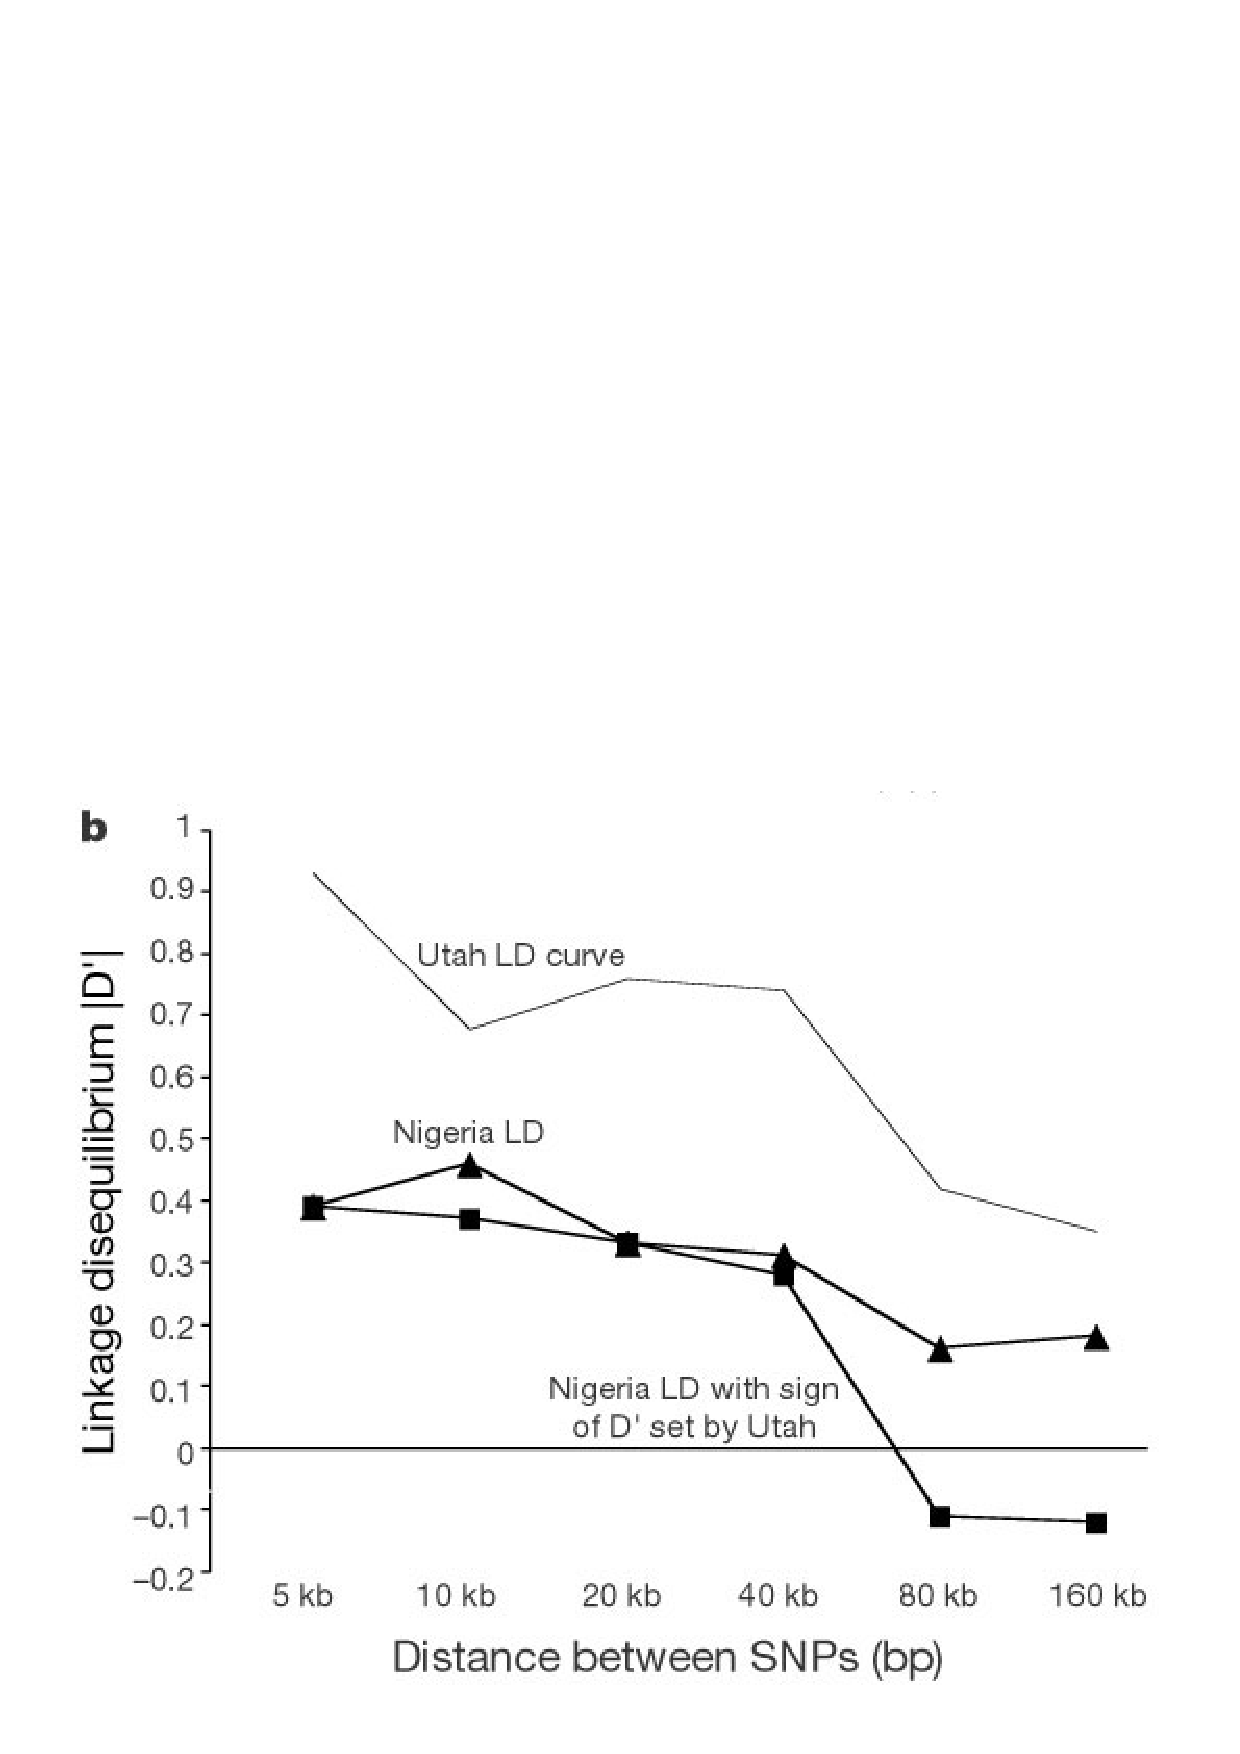
\includegraphics[height=0.85\textheight]{ldcurve.jpg}
\column{0.4\textwidth}
\raggedright
\begin{itemize}
\item LD declines with distance along chromosome
\item More LD in Europe than Africa
\item Why?
\end{itemize}
\textsc{\footnotesize (Reich et al 2001)}
\end{columns}
\end{frame}

\begin{frame}
\frametitle{LD unevenly distributed within genome}
\centering
 \includegraphics[height=0.85\textheight]{voight-loci.png}
\end{frame}

\begin{frame}
\frametitle{Facts we need to understand}
\begin{itemize}
\item LD decays w/ distance along chromosome.
\item Populations differ.
\item Unevenly distributed w/i genome
\end{itemize}
\end{frame}

\begin{frame}
\frametitle{Cross-overs shuffle DNA}
\begin{columns}
\column{0.6\textwidth}
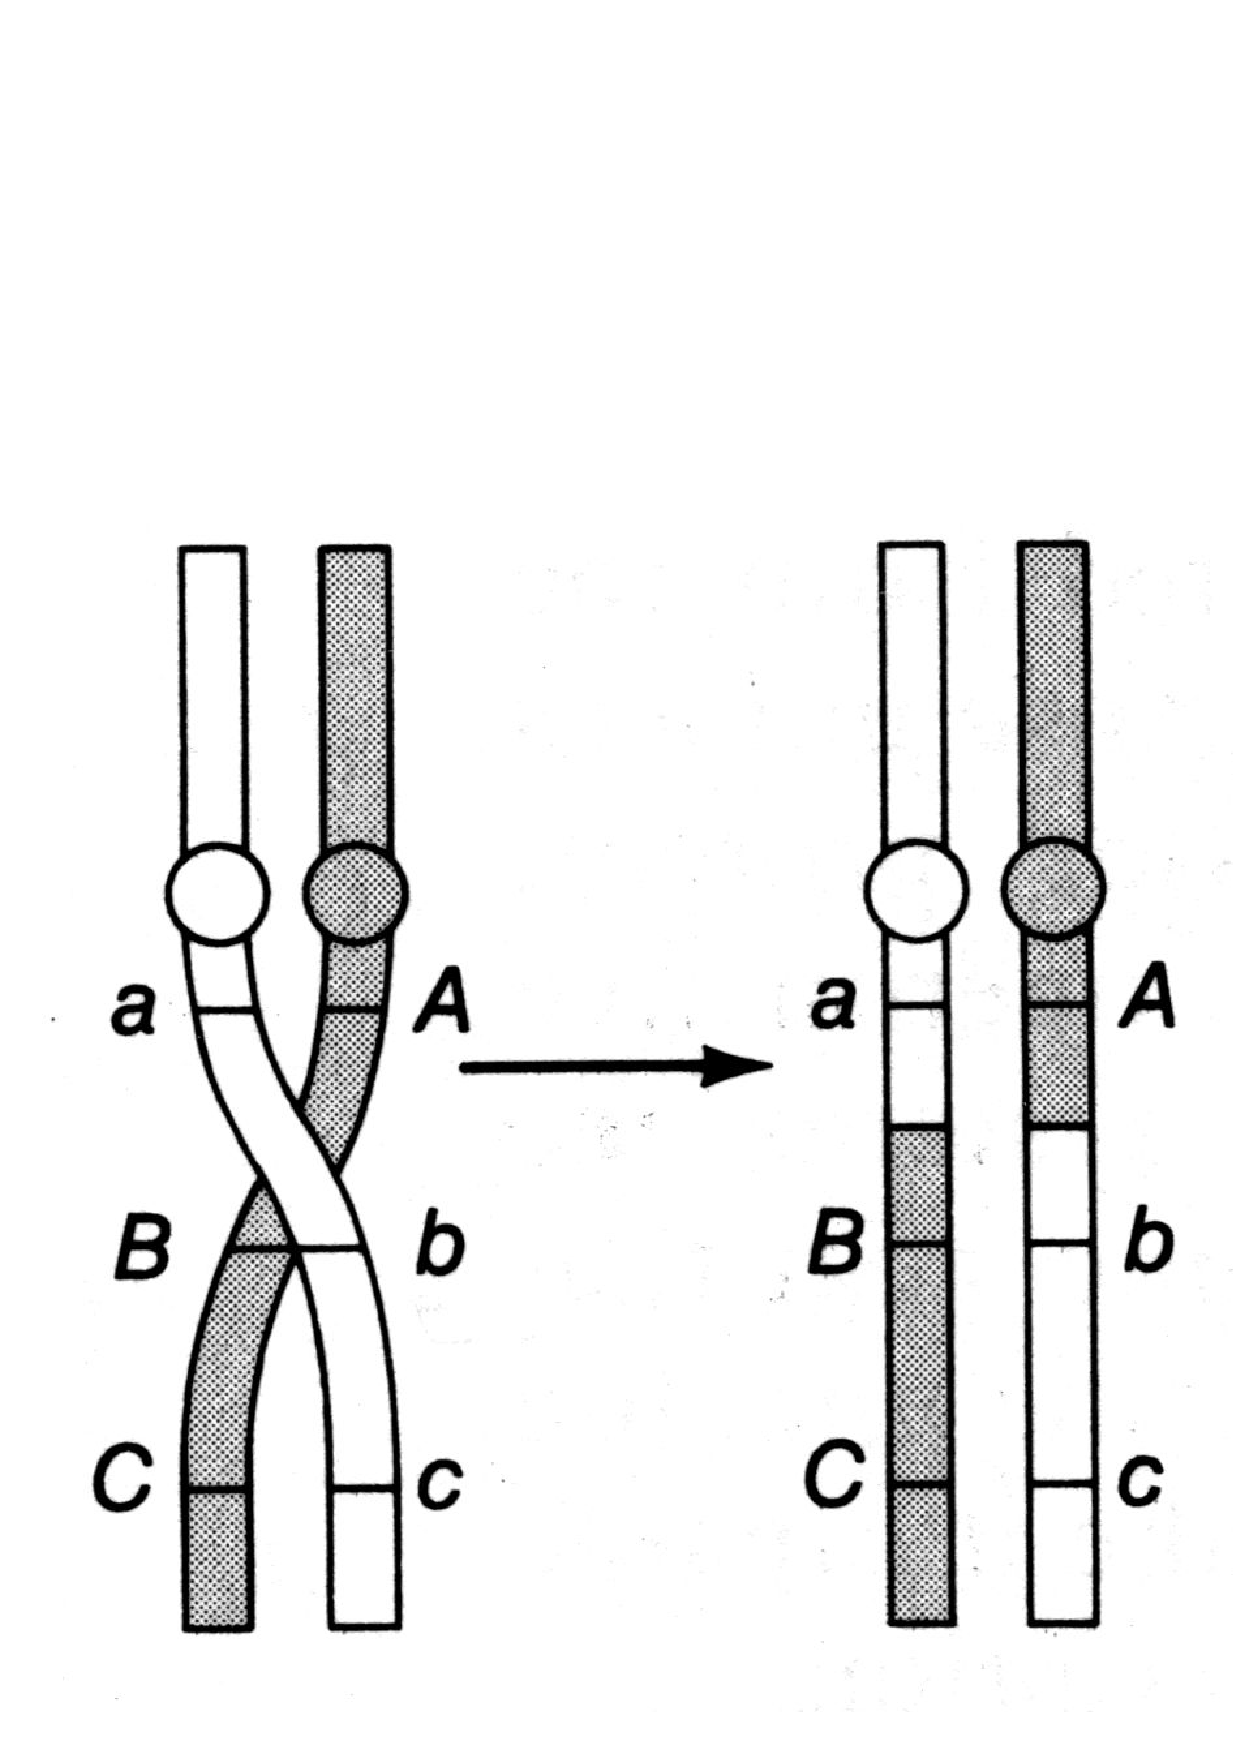
\includegraphics[width=\textwidth]{crossover.pdf}
\column{0.4\textwidth}
\raggedright
\begin{itemize}
\item occur during reproduction.
\item shuffle parental chromosomes.
\item sites far apart more likely to recombine
\item result: ``recombinant'' chromosomes
\end{itemize}
\end{columns}
\end{frame}

\begin{frame}[containsverbatim]
\frametitle{Why loci are independent on recombinants}
\begin{verbatim}
 __________________________________________________
|                                                  |
|.....A........b.....   A recombinant chromosome.  |
|\________/\________/                              |
| from dad  from mom                               |
|                                                  |
|                       Gamete from Dad carried A. |
|                       Gamete from Mom carried b. |
|                                                  |
|Probability of this?   p_A p_b under random mating|
|__________________________________________________|
\end{verbatim}
\end{frame}

\begin{frame}
\frametitle{Ingredients of a model}

{\centering\fbox{\begin{minipage}{0.9\textwidth}
\begin{eqnarray*}
x_1 &=& \hbox{frequency of $AB$-gametes among parents}\\
p_A &=& \hbox{frequency of $A$-gametes among parents}\\
p_B &=& \hbox{frequency of $B$-gametes among parents}\\
c   &=& \hbox{prob of recombination between the two loci}
\end{eqnarray*}
\end{minipage}}\\}

\bigskip\pause

In any generation, there are two kinds of $AB$ gamete:
\begin{enumerate}
\item non-recombinants: these were $AB$s in the last generation
  \pause    Frequency: $(1-c)x_1$
\pause
\item recombinants: formed from an $A$ gamete and a $B$ gamete, drawn
  at random.  \pause Frequency: $cp_A p_B$
\end{enumerate}
\pause
Next step: sum these contributions.
\end{frame}

\frame{\frametitle{Model with random mating, no selection}

{\centering\fbox{\begin{minipage}{0.9\textwidth}
\begin{eqnarray*}
x_1 &=& \hbox{frequency of $AB$-gametes among parents}\\
p_A &=& \hbox{frequency of $A$-gametes among parents}\\
p_B &=& \hbox{frequency of $B$-gametes among parents}\\
c   &=& \hbox{prob of recombination between the two loci}
\end{eqnarray*}
\end{minipage}}\\}

\bigskip

Change in frequency of $AB$-gametes during one generation:
\begin{eqnarray*}
x'_1 &=& \overbrace{(1-c)x_1}^{\hbox{\small nonrecombinants}}
+ \overbrace{\mathstrut c p_A p_B}^{\hbox{\small recombinants}}\\
\pause
  &=& x_1 - c(x_1 - p_A p_B)\\
\pause
  &=& x_1 -cD
\end{eqnarray*}
}

\begin{frame}
\frametitle{Several equivalent definitions of $D$}
The previous slide defined $D$, a measure of LD:
\[
\begin{array}{crcl}
\hbox{Gamete}     & \multicolumn{3}{c}{\hbox{Definition}}\\
AB & D &=& x_1 - p_A p_B\\
\pause
Ab & -D &=& x_2 - p_A p_b\\
\pause
aB & -D &=& x_3 - p_a p_B\\
ab & D &=& x_4 - p_a p_b\\
\end{array}
\]
\pause
If the association between $A$ and $B$ is positive, then that between
$A$ and $b$ must be negative.
\pause
A more convenient formula:
\[
D = x_1x_4 - x_2x_3
\]
They all give the same answer.
\end{frame}

\begin{frame}
\frametitle{Calculating $D$}
\begin{columns}
\column{0.35\textwidth}
\centering
\begin{tabular}{ccc}
       & \multicolumn{2}{c}{Locus}\\
Gamete &  1 & 2\\ \hline
 1&A&B\\
 2&A&B\\
 3&A&B\\
 4&A&B\\
 5&A&B\\
 6&A&b\\
 7&a&B\\
 8&a&B\\
 9&a&b\\
10&a&b\\
\end{tabular}
\column{0.65\textwidth}
\centering
\begin{tabular}{cccc}
AB & Ab & aB & ab\\
$x_1$ & $x_2$ & $x_3$ & $x_4$
\end{tabular}\\

\pause
\bigskip

\begin{tabular}{c|cc|c}
 \multicolumn{1}{c}{} & A & \multicolumn{1}{c}{a}\\
\cline{2-3}
B & 5 & 2 & 7\\
b & 1 & 2 & 3\\
\cline{2-3}
\multicolumn{1}{c}{}
  & 6 & \multicolumn{1}{c}{4} & 10
\end{tabular}\\
\pause
\begin{eqnarray*}
D &=& x_1x_4 - x_2x_3\\ \pause
  &=& \frac{5}{10} \cdot \frac{2}{10} - \frac{1}{10}\cdot\frac{2}{10}\\
\pause
  &=& \frac{2}{25}
\end{eqnarray*}
\end{columns}
\end{frame}

\begin{frame}
\frametitle{All four gametes, still no selection}
\[
\begin{array}{crcl}
\hbox{Gamete}     & \multicolumn{3}{c}{Recurrence}\\
AB & x'_1 &=& x_1 -cD\\
Ab & x'_2 &=& x_2 +cD\\
aB & x'_3 &=& x_3 +cD\\
ab & x'_4 &=& x_4 -cD\\
\end{array}
\]
\end{frame}

\begin{frame}
\frametitle{How recombination affects $D$}
After one generation,
\begin{eqnarray*}
D' &=& x'_1 x'_4 - x'_2 x'_3\\
   &=& (x_1 -cD)(x_4-cD) - (x_2+cD)(x_3+cD)\\
   &=& (1-c)D
\end{eqnarray*}
$D$ declines each generation by a factor of $1-c$.

\pause
After $t$ generations,
\[
D_t = D_0 (1-c)^t
\]
\end{frame}

\begin{frame}
\frametitle{$D$ declines gradually toward zero}
\begin{columns}
\column{0.6\textwidth}
%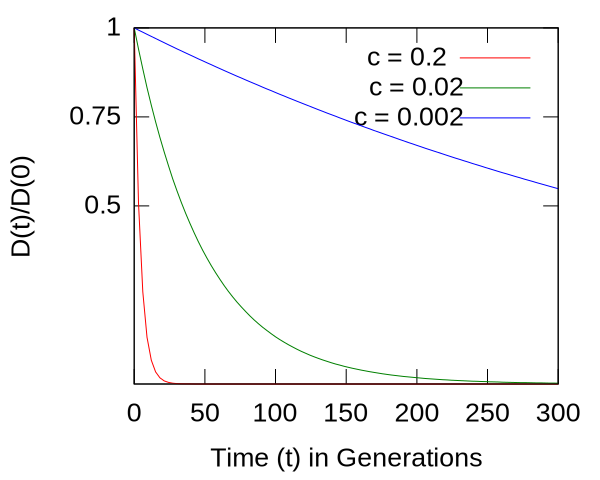
\includegraphics[width=\textwidth]{lddecay.pdf}
% GNUPLOT: LaTeX picture
\setlength{\unitlength}{0.240900pt}
\ifx\plotpoint\undefined\newsavebox{\plotpoint}\fi
\sbox{\plotpoint}{\rule[-0.200pt]{0.400pt}{0.400pt}}%
\begin{picture}(840,749)(0,0)
\sbox{\plotpoint}{\rule[-0.200pt]{0.400pt}{0.400pt}}%
\put(191.0,276.0){\rule[-0.200pt]{4.818pt}{0.400pt}}
\put(171,276){\makebox(0,0)[r]{ 0.25}}
\put(759.0,276.0){\rule[-0.200pt]{4.818pt}{0.400pt}}
\put(191.0,420.0){\rule[-0.200pt]{4.818pt}{0.400pt}}
\put(171,420){\makebox(0,0)[r]{ 0.5}}
\put(759.0,420.0){\rule[-0.200pt]{4.818pt}{0.400pt}}
\put(191.0,565.0){\rule[-0.200pt]{4.818pt}{0.400pt}}
\put(171,565){\makebox(0,0)[r]{ 0.75}}
\put(759.0,565.0){\rule[-0.200pt]{4.818pt}{0.400pt}}
\put(191.0,709.0){\rule[-0.200pt]{4.818pt}{0.400pt}}
\put(171,709){\makebox(0,0)[r]{ 1}}
\put(759.0,709.0){\rule[-0.200pt]{4.818pt}{0.400pt}}
\put(191.0,131.0){\rule[-0.200pt]{0.400pt}{4.818pt}}
\put(191,90){\makebox(0,0){ 0}}
\put(191.0,689.0){\rule[-0.200pt]{0.400pt}{4.818pt}}
\put(289.0,131.0){\rule[-0.200pt]{0.400pt}{4.818pt}}
\put(289,90){\makebox(0,0){ 50}}
\put(289.0,689.0){\rule[-0.200pt]{0.400pt}{4.818pt}}
\put(387.0,131.0){\rule[-0.200pt]{0.400pt}{4.818pt}}
\put(387,90){\makebox(0,0){ 100}}
\put(387.0,689.0){\rule[-0.200pt]{0.400pt}{4.818pt}}
\put(485.0,131.0){\rule[-0.200pt]{0.400pt}{4.818pt}}
\put(485,90){\makebox(0,0){ 150}}
\put(485.0,689.0){\rule[-0.200pt]{0.400pt}{4.818pt}}
\put(583.0,131.0){\rule[-0.200pt]{0.400pt}{4.818pt}}
\put(583,90){\makebox(0,0){ 200}}
\put(583.0,689.0){\rule[-0.200pt]{0.400pt}{4.818pt}}
\put(681.0,131.0){\rule[-0.200pt]{0.400pt}{4.818pt}}
\put(681,90){\makebox(0,0){ 250}}
\put(681.0,689.0){\rule[-0.200pt]{0.400pt}{4.818pt}}
\put(779.0,131.0){\rule[-0.200pt]{0.400pt}{4.818pt}}
\put(779,90){\makebox(0,0){ 300}}
\put(779.0,689.0){\rule[-0.200pt]{0.400pt}{4.818pt}}
\put(191.0,131.0){\rule[-0.200pt]{0.400pt}{139.240pt}}
\put(191.0,131.0){\rule[-0.200pt]{141.649pt}{0.400pt}}
\put(779.0,131.0){\rule[-0.200pt]{0.400pt}{139.240pt}}
\put(191.0,709.0){\rule[-0.200pt]{141.649pt}{0.400pt}}
\put(30,420){\makebox(0,0){\Large$\frac{D_t}{D_0}$}}
\put(485,29){\makebox(0,0){Time (t) in Generations}}
\put(619,669){\makebox(0,0)[r]{c = 0.2}}
\put(639.0,669.0){\rule[-0.200pt]{24.090pt}{0.400pt}}
\put(191,709){\usebox{\plotpoint}}
\multiput(191.59,629.99)(0.482,-25.624){9}{\rule{0.116pt}{19.033pt}}
\multiput(190.17,669.50)(6.000,-244.495){2}{\rule{0.400pt}{9.517pt}}
\multiput(197.59,384.46)(0.482,-13.057){9}{\rule{0.116pt}{9.767pt}}
\multiput(196.17,404.73)(6.000,-124.729){2}{\rule{0.400pt}{4.883pt}}
\multiput(203.59,259.38)(0.482,-6.548){9}{\rule{0.116pt}{4.967pt}}
\multiput(202.17,269.69)(6.000,-62.691){2}{\rule{0.400pt}{2.483pt}}
\multiput(209.59,196.35)(0.482,-3.293){9}{\rule{0.116pt}{2.567pt}}
\multiput(208.17,201.67)(6.000,-31.673){2}{\rule{0.400pt}{1.283pt}}
\multiput(215.59,164.33)(0.482,-1.666){9}{\rule{0.116pt}{1.367pt}}
\multiput(214.17,167.16)(6.000,-16.163){2}{\rule{0.400pt}{0.683pt}}
\multiput(221.59,147.82)(0.482,-0.852){9}{\rule{0.116pt}{0.767pt}}
\multiput(220.17,149.41)(6.000,-8.409){2}{\rule{0.400pt}{0.383pt}}
\multiput(227.00,139.93)(0.599,-0.477){7}{\rule{0.580pt}{0.115pt}}
\multiput(227.00,140.17)(4.796,-5.000){2}{\rule{0.290pt}{0.400pt}}
\put(233,134.17){\rule{1.300pt}{0.400pt}}
\multiput(233.00,135.17)(3.302,-2.000){2}{\rule{0.650pt}{0.400pt}}
\put(239,132.17){\rule{1.100pt}{0.400pt}}
\multiput(239.00,133.17)(2.717,-2.000){2}{\rule{0.550pt}{0.400pt}}
\put(250,130.67){\rule{1.445pt}{0.400pt}}
\multiput(250.00,131.17)(3.000,-1.000){2}{\rule{0.723pt}{0.400pt}}
\put(244.0,132.0){\rule[-0.200pt]{1.445pt}{0.400pt}}
\put(256.0,131.0){\rule[-0.200pt]{125.991pt}{0.400pt}}
\put(619,628){\makebox(0,0)[r]{c = 0.02}}
\multiput(639,628)(20.756,0.000){5}{\usebox{\plotpoint}}
\put(739,628){\usebox{\plotpoint}}
\put(191,709){\usebox{\plotpoint}}
\multiput(191,709)(3.607,-20.440){2}{\usebox{\plotpoint}}
\multiput(197,675)(3.713,-20.421){2}{\usebox{\plotpoint}}
\put(205.93,627.33){\usebox{\plotpoint}}
\multiput(209,612)(4.205,-20.325){2}{\usebox{\plotpoint}}
\put(218.83,566.42){\usebox{\plotpoint}}
\put(223.49,546.20){\usebox{\plotpoint}}
\put(228.30,526.01){\usebox{\plotpoint}}
\multiput(233,508)(5.239,-20.083){2}{\usebox{\plotpoint}}
\put(243.61,465.66){\usebox{\plotpoint}}
\put(249.47,445.75){\usebox{\plotpoint}}
\put(255.99,426.04){\usebox{\plotpoint}}
\put(262.61,406.37){\usebox{\plotpoint}}
\put(269.90,386.94){\usebox{\plotpoint}}
\put(277.57,367.66){\usebox{\plotpoint}}
\put(285.75,348.58){\usebox{\plotpoint}}
\put(294.59,329.81){\usebox{\plotpoint}}
\put(304.29,311.46){\usebox{\plotpoint}}
\put(314.55,293.42){\usebox{\plotpoint}}
\put(325.48,275.78){\usebox{\plotpoint}}
\put(337.29,258.74){\usebox{\plotpoint}}
\put(350.41,242.69){\usebox{\plotpoint}}
\put(364.51,227.49){\usebox{\plotpoint}}
\put(379.67,213.33){\usebox{\plotpoint}}
\put(396.20,200.87){\usebox{\plotpoint}}
\put(413.47,189.35){\usebox{\plotpoint}}
\put(431.77,179.61){\usebox{\plotpoint}}
\put(450.46,170.77){\usebox{\plotpoint}}
\put(470.06,163.98){\usebox{\plotpoint}}
\put(489.75,157.42){\usebox{\plotpoint}}
\put(509.90,152.70){\usebox{\plotpoint}}
\put(530.29,148.94){\usebox{\plotpoint}}
\put(550.73,145.38){\usebox{\plotpoint}}
\put(571.21,142.00){\usebox{\plotpoint}}
\put(591.84,140.53){\usebox{\plotpoint}}
\put(612.40,138.10){\usebox{\plotpoint}}
\put(633.06,137.00){\usebox{\plotpoint}}
\put(653.74,136.00){\usebox{\plotpoint}}
\put(674.41,135.00){\usebox{\plotpoint}}
\put(695.08,134.00){\usebox{\plotpoint}}
\put(715.81,133.70){\usebox{\plotpoint}}
\put(736.51,133.00){\usebox{\plotpoint}}
\put(757.26,133.00){\usebox{\plotpoint}}
\put(777.94,132.00){\usebox{\plotpoint}}
\put(779,132){\usebox{\plotpoint}}
\sbox{\plotpoint}{\rule[-0.500pt]{1.000pt}{1.000pt}}%
\sbox{\plotpoint}{\rule[-0.200pt]{0.400pt}{0.400pt}}%
\put(619,587){\makebox(0,0)[r]{c = 0.002}}
\sbox{\plotpoint}{\rule[-0.500pt]{1.000pt}{1.000pt}}%
\multiput(639,587)(41.511,0.000){3}{\usebox{\plotpoint}}
\put(739,587){\usebox{\plotpoint}}
\put(191,709){\usebox{\plotpoint}}
\put(191.00,709.00){\usebox{\plotpoint}}
\put(226.79,688.14){\usebox{\plotpoint}}
\put(262.73,667.63){\usebox{\plotpoint}}
\put(299.41,648.30){\usebox{\plotpoint}}
\put(336.43,629.54){\usebox{\plotpoint}}
\put(373.45,610.77){\usebox{\plotpoint}}
\put(410.92,593.04){\usebox{\plotpoint}}
\put(448.31,575.23){\usebox{\plotpoint}}
\put(486.24,558.59){\usebox{\plotpoint}}
\put(524.50,542.75){\usebox{\plotpoint}}
\put(562.49,526.25){\usebox{\plotpoint}}
\put(600.99,511.00){\usebox{\plotpoint}}
\put(639.68,496.16){\usebox{\plotpoint}}
\put(678.56,481.81){\usebox{\plotpoint}}
\put(717.94,468.69){\usebox{\plotpoint}}
\put(757.21,455.26){\usebox{\plotpoint}}
\put(779,448){\usebox{\plotpoint}}
\sbox{\plotpoint}{\rule[-0.200pt]{0.400pt}{0.400pt}}%
\put(191.0,131.0){\rule[-0.200pt]{0.400pt}{139.240pt}}
\put(191.0,131.0){\rule[-0.200pt]{141.649pt}{0.400pt}}
\put(779.0,131.0){\rule[-0.200pt]{0.400pt}{139.240pt}}
\put(191.0,709.0){\rule[-0.200pt]{141.649pt}{0.400pt}}
\end{picture}

\column{0.4\textwidth}
\begin{block}{$c=0.2$}
\begin{itemize}
\item Loci far apart
\item Loose linkage
\item LD declines rapidly
\end{itemize}
\end{block}
\begin{block}{$c=0.02$}<2->
\begin{itemize}
\item Loci closer
\item slower decline
\end{itemize}
\end{block}
\begin{block}{$c=0.002$}<3->
\begin{itemize}
\item Loci closer still
\item even slower decline
\end{itemize}
\end{block}
\end{columns}
\end{frame}

\begin{frame}
Is this theory enough to explain the data?
\end{frame}

\begin{frame}
\frametitle{More LD in Europe than Africa}
\begin{columns}
\column{0.6\textwidth}
 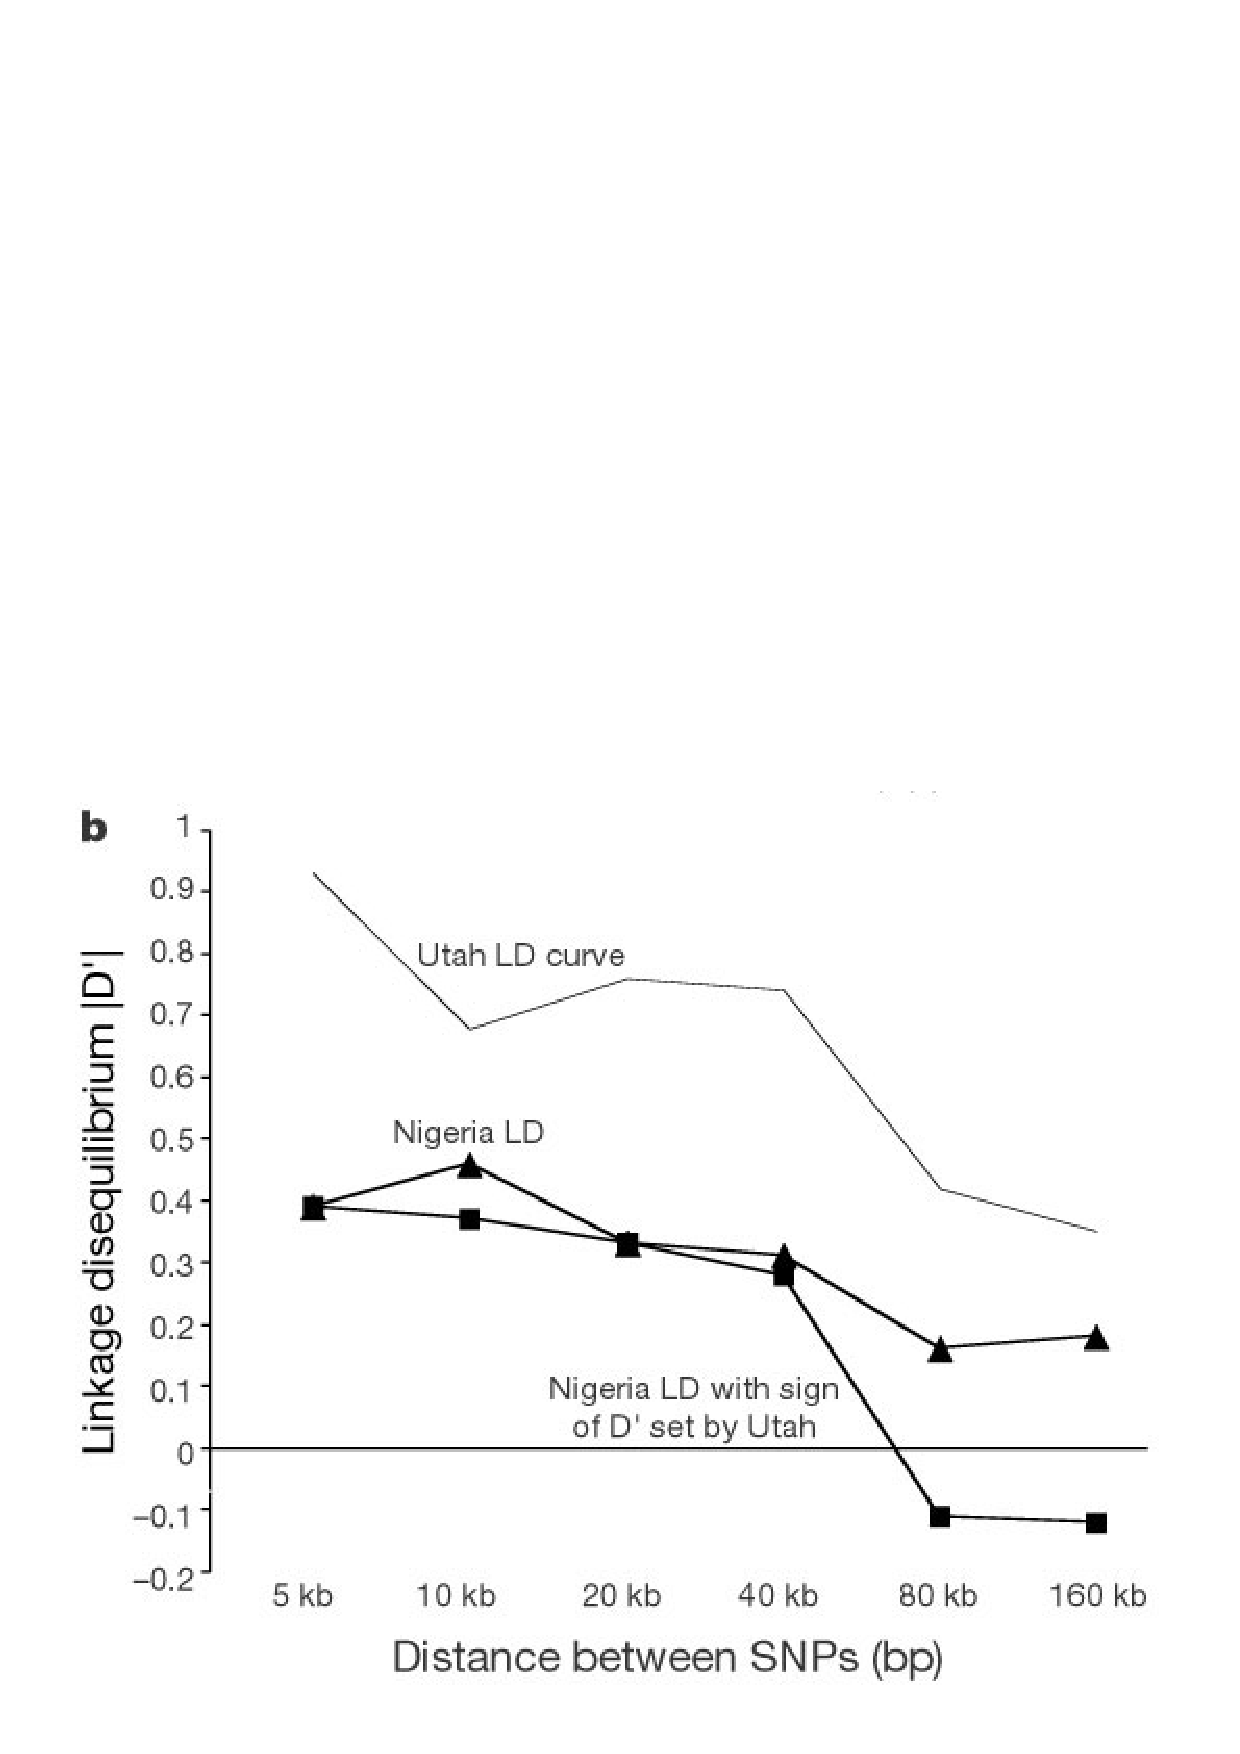
\includegraphics[height=0.85\textheight]{ldcurve.jpg}
\column{0.4\textwidth}
\raggedright
\begin{itemize}
\item $c$ increases w/ distance along chromosome.
\item Therefore LD should decline.
\item But why more LD in Europe?
\end{itemize}
\textsc{\footnotesize (Reich et al 2001)}
\end{columns}
\end{frame}

\begin{frame}
\begin{columns}
\column{0.6\textwidth}
 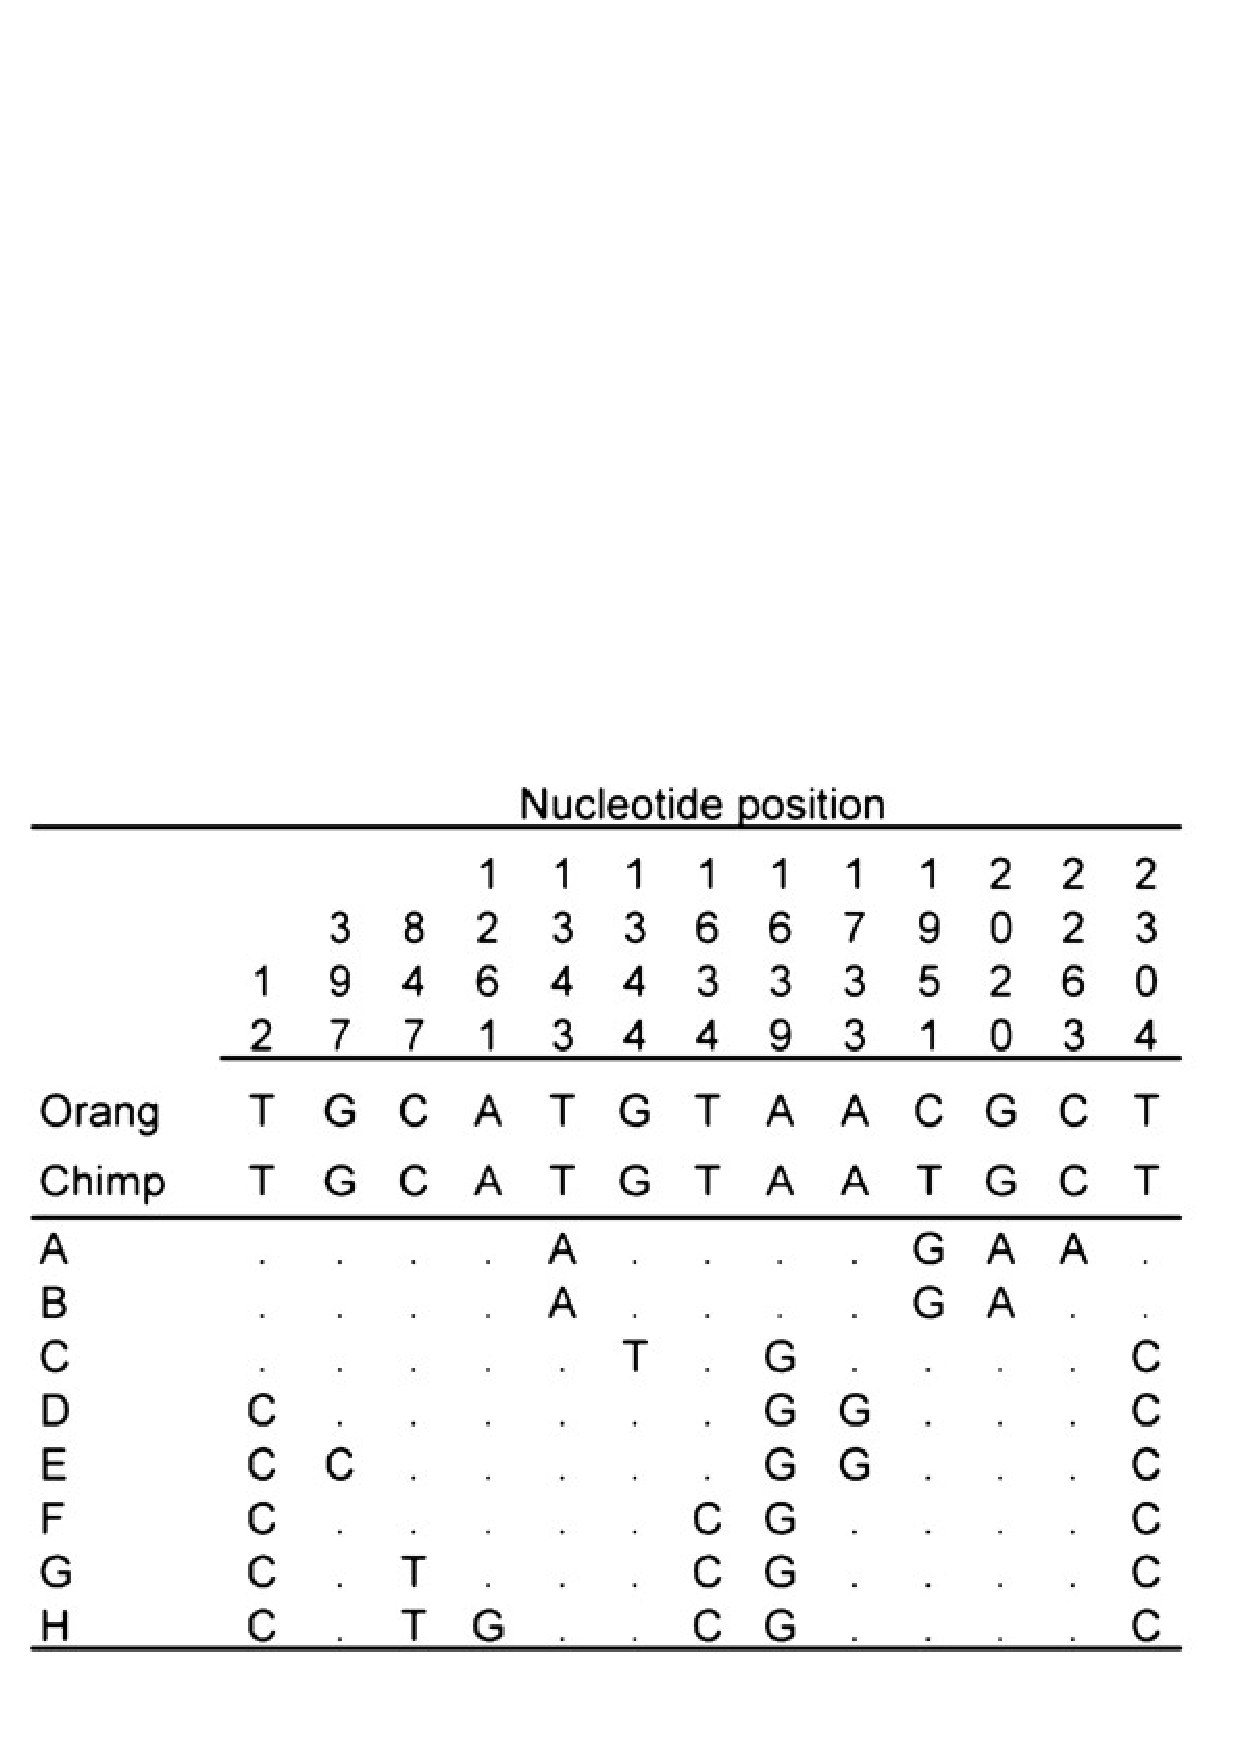
\includegraphics[width=\textwidth]{rrm2p4seq.png}\\
\textsc{\footnotesize (Garrigan et al 2004)}
\column{0.4\textwidth}\raggedright
\begin{itemize}
\item Short DNA sequence.
\item tight linkage: $c$ is small
\item LD decays very slowly
\item But why is it not zero?
\end{itemize}
\end{columns}
\end{frame}

\begin{frame}
\begin{columns}
\column{0.6\textwidth}
 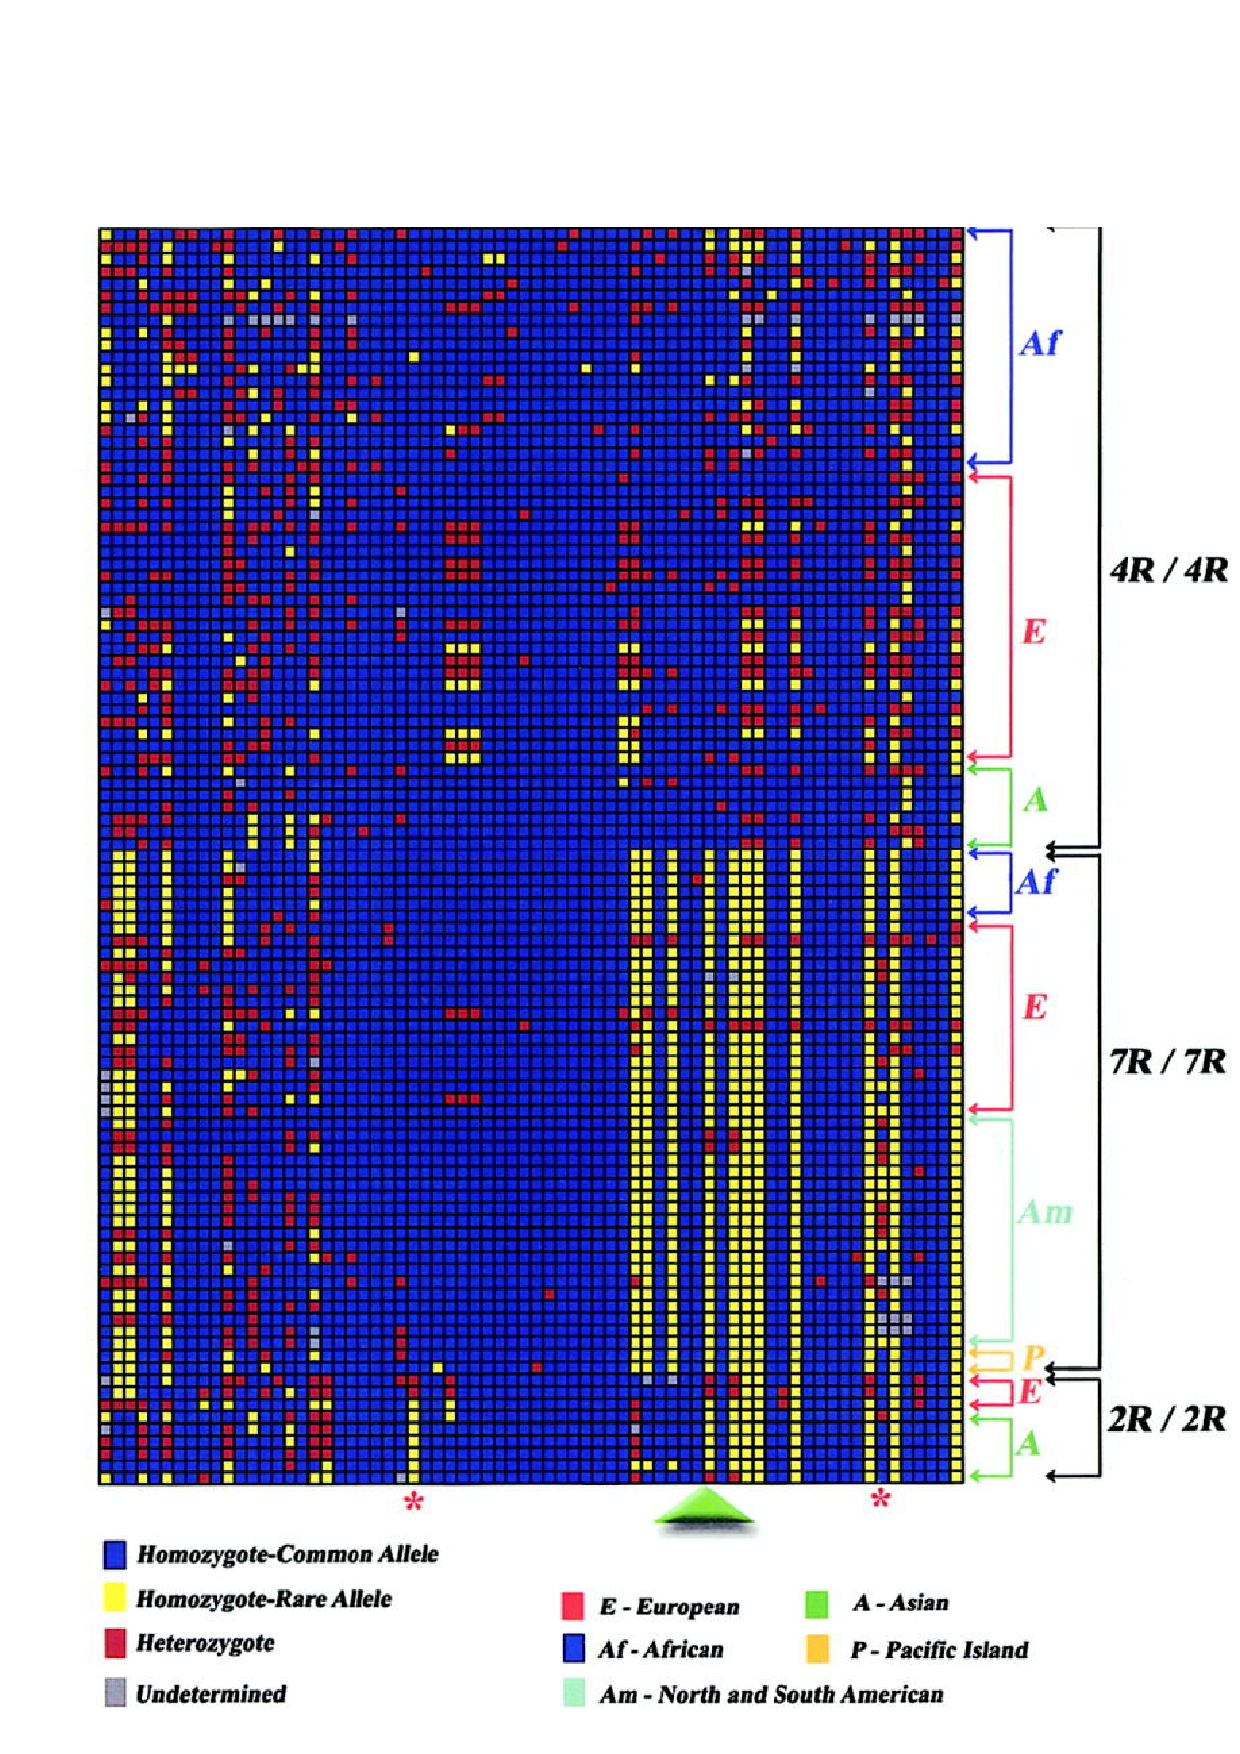
\includegraphics[height=0.9\textheight]{drd4-polymorph.pdf}
\column{0.4\textwidth}\raggedright
\begin{itemize}
\item Also a short sequence
\item But why is there any LD?
\end{itemize}
\end{columns}
\end{frame}

\begin{frame}
\frametitle{Why is LD unevenly distributed?}
\centering
 \includegraphics[height=0.85\textheight]{voight-loci.png}
\end{frame}

\begin{frame}
\frametitle{Summary}
\begin{itemize}
\item Our theory explains why $D$ declines w/ distance along
  chromosome.
\item If loci are far apart on chromosome, $c$ is high and $D$
  declines rapidly.
\item It tells us nothing about the forces that generate LD.
\item Nothing about population differences.
\item Nothing about variation across the genome.
\end{itemize}
\end{frame}
\end{document}

